\documentclass[twoside]{book}

% Packages required by doxygen
\usepackage{fixltx2e}
\usepackage{calc}
\usepackage{doxygen}
\usepackage[export]{adjustbox} % also loads graphicx
\usepackage{graphicx}
\usepackage[utf8]{inputenc}
\usepackage{makeidx}
\usepackage{multicol}
\usepackage{multirow}
\PassOptionsToPackage{warn}{textcomp}
\usepackage{textcomp}
\usepackage[nointegrals]{wasysym}
\usepackage[table]{xcolor}

% Font selection
\usepackage[T1]{fontenc}
\usepackage[scaled=.90]{helvet}
\usepackage{courier}
\usepackage{amssymb}
\usepackage{sectsty}
\renewcommand{\familydefault}{\sfdefault}
\allsectionsfont{%
  \fontseries{bc}\selectfont%
  \color{darkgray}%
}
\renewcommand{\DoxyLabelFont}{%
  \fontseries{bc}\selectfont%
  \color{darkgray}%
}
\newcommand{\+}{\discretionary{\mbox{\scriptsize$\hookleftarrow$}}{}{}}

% Page & text layout
\usepackage{geometry}
\geometry{%
  a4paper,%
  top=2.5cm,%
  bottom=2.5cm,%
  left=2.5cm,%
  right=2.5cm%
}
\tolerance=750
\hfuzz=15pt
\hbadness=750
\setlength{\emergencystretch}{15pt}
\setlength{\parindent}{0cm}
\setlength{\parskip}{3ex plus 2ex minus 2ex}
\makeatletter
\renewcommand{\paragraph}{%
  \@startsection{paragraph}{4}{0ex}{-1.0ex}{1.0ex}{%
    \normalfont\normalsize\bfseries\SS@parafont%
  }%
}
\renewcommand{\subparagraph}{%
  \@startsection{subparagraph}{5}{0ex}{-1.0ex}{1.0ex}{%
    \normalfont\normalsize\bfseries\SS@subparafont%
  }%
}
\makeatother

% Headers & footers
\usepackage{fancyhdr}
\pagestyle{fancyplain}
\fancyhead[LE]{\fancyplain{}{\bfseries\thepage}}
\fancyhead[CE]{\fancyplain{}{}}
\fancyhead[RE]{\fancyplain{}{\bfseries\leftmark}}
\fancyhead[LO]{\fancyplain{}{\bfseries\rightmark}}
\fancyhead[CO]{\fancyplain{}{}}
\fancyhead[RO]{\fancyplain{}{\bfseries\thepage}}
\fancyfoot[LE]{\fancyplain{}{}}
\fancyfoot[CE]{\fancyplain{}{}}
\fancyfoot[RE]{\fancyplain{}{\bfseries\scriptsize Generated by Doxygen }}
\fancyfoot[LO]{\fancyplain{}{\bfseries\scriptsize Generated by Doxygen }}
\fancyfoot[CO]{\fancyplain{}{}}
\fancyfoot[RO]{\fancyplain{}{}}
\renewcommand{\footrulewidth}{0.4pt}
\renewcommand{\chaptermark}[1]{%
  \markboth{#1}{}%
}
\renewcommand{\sectionmark}[1]{%
  \markright{\thesection\ #1}%
}

% Indices & bibliography
\usepackage{natbib}
\usepackage[titles]{tocloft}
\setcounter{tocdepth}{3}
\setcounter{secnumdepth}{5}
\makeindex

% Hyperlinks (required, but should be loaded last)
\usepackage{ifpdf}
\ifpdf
  \usepackage[pdftex,pagebackref=true]{hyperref}
\else
  \usepackage[ps2pdf,pagebackref=true]{hyperref}
\fi
\hypersetup{%
  colorlinks=true,%
  linkcolor=blue,%
  citecolor=blue,%
  unicode%
}

% Custom commands
\newcommand{\clearemptydoublepage}{%
  \newpage{\pagestyle{empty}\cleardoublepage}%
}

\usepackage{caption}
\captionsetup{labelsep=space,justification=centering,font={bf},singlelinecheck=off,skip=4pt,position=top}

%===== C O N T E N T S =====

\begin{document}

% Titlepage & ToC
\hypersetup{pageanchor=false,
             bookmarksnumbered=true,
             pdfencoding=unicode
            }
\pagenumbering{alph}
\begin{titlepage}
\vspace*{7cm}
\begin{center}%
{\Large Omega \\[1ex]\large 0.\+0.\+1 }\\
\vspace*{1cm}
{\large Generated by Doxygen 1.8.14}\\
\end{center}
\end{titlepage}
\clearemptydoublepage
\pagenumbering{roman}
\tableofcontents
\clearemptydoublepage
\pagenumbering{arabic}
\hypersetup{pageanchor=true}

%--- Begin generated contents ---
\chapter{Hierarchical Index}
\section{Class Hierarchy}
This inheritance list is sorted roughly, but not completely, alphabetically\+:\begin{DoxyCompactList}
\item \contentsline{section}{edge}{\pageref{structedge}}{}
\item \contentsline{section}{element\+Manager}{\pageref{classelement_manager}}{}
\item \contentsline{section}{material\+Manager}{\pageref{classmaterial_manager}}{}
\begin{DoxyCompactList}
\item \contentsline{section}{dsid}{\pageref{classdsid}}{}
\item \contentsline{section}{isotropic\+Elastic}{\pageref{classisotropic_elastic}}{}
\end{DoxyCompactList}
\item \contentsline{section}{node}{\pageref{structnode}}{}
\item \contentsline{section}{solver\+Manager}{\pageref{classsolver_manager}}{}
\item \contentsline{section}{surface}{\pageref{structsurface}}{}
\item \contentsline{section}{task\+Manager}{\pageref{classtask_manager}}{}
\end{DoxyCompactList}

\chapter{Class Index}
\section{Class List}
Here are the classes, structs, unions and interfaces with brief descriptions\+:\begin{DoxyCompactList}
\item\contentsline{section}{\hyperlink{classdsid}{dsid} }{\pageref{classdsid}}{}
\item\contentsline{section}{\hyperlink{structedge}{edge} }{\pageref{structedge}}{}
\item\contentsline{section}{\hyperlink{classelement_manager}{element\+Manager} }{\pageref{classelement_manager}}{}
\item\contentsline{section}{\hyperlink{class_ellipse}{Ellipse} }{\pageref{class_ellipse}}{}
\item\contentsline{section}{\hyperlink{classisotropic_elastic}{isotropic\+Elastic} }{\pageref{classisotropic_elastic}}{}
\item\contentsline{section}{\hyperlink{classmaterial}{material} }{\pageref{classmaterial}}{}
\item\contentsline{section}{\hyperlink{classmaterial_factory}{material\+Factory} }{\pageref{classmaterial_factory}}{}
\item\contentsline{section}{\hyperlink{structmaterial_factory_register}{material\+Factory\+Register$<$ T $>$} }{\pageref{structmaterial_factory_register}}{}
\item\contentsline{section}{\hyperlink{classmaterial_manager}{material\+Manager} }{\pageref{classmaterial_manager}}{}
\item\contentsline{section}{\hyperlink{structnode}{node} }{\pageref{structnode}}{}
\item\contentsline{section}{\hyperlink{classshape_function}{shape\+Function} }{\pageref{classshape_function}}{}
\item\contentsline{section}{\hyperlink{classshape_function_factory}{shape\+Function\+Factory} }{\pageref{classshape_function_factory}}{}
\item\contentsline{section}{\hyperlink{structshape_function_factory_register}{shape\+Function\+Factory\+Register$<$ T $>$} }{\pageref{structshape_function_factory_register}}{}
\item\contentsline{section}{\hyperlink{classshape_function_manager}{shape\+Function\+Manager} }{\pageref{classshape_function_manager}}{}
\item\contentsline{section}{\hyperlink{classsolver_manager}{solver\+Manager} }{\pageref{classsolver_manager}}{}
\item\contentsline{section}{\hyperlink{class_square}{Square} }{\pageref{class_square}}{}
\item\contentsline{section}{\hyperlink{structsurface}{surface} }{\pageref{structsurface}}{}
\item\contentsline{section}{\hyperlink{classtask_manager}{task\+Manager} }{\pageref{classtask_manager}}{}
\end{DoxyCompactList}

\chapter{File Index}
\section{File List}
Here is a list of all documented files with brief descriptions\+:\begin{DoxyCompactList}
\item\contentsline{section}{/\+Users/haoxu/\+Documents/git/element/{\bfseries edge.\+h} }{\pageref{edge_8h}}{}
\item\contentsline{section}{/\+Users/haoxu/\+Documents/git/element/{\bfseries node.\+h} }{\pageref{node_8h}}{}
\item\contentsline{section}{/\+Users/haoxu/\+Documents/git/element/{\bfseries shape\+Function.\+h} }{\pageref{shape_function_8h}}{}
\item\contentsline{section}{/\+Users/haoxu/\+Documents/git/element/{\bfseries shape\+Function\+Factory.\+h} }{\pageref{shape_function_factory_8h}}{}
\item\contentsline{section}{/\+Users/haoxu/\+Documents/git/element/{\bfseries surface.\+h} }{\pageref{surface_8h}}{}
\item\contentsline{section}{/\+Users/haoxu/\+Documents/git/\+Omega/src/class\+Manager/\hyperlink{element_manager_8h}{element\+Manager.\+h} }{\pageref{element_manager_8h}}{}
\item\contentsline{section}{/\+Users/haoxu/\+Documents/git/\+Omega/src/class\+Manager/\hyperlink{material_manager_8h}{material\+Manager.\+h} }{\pageref{material_manager_8h}}{}
\item\contentsline{section}{/\+Users/haoxu/\+Documents/git/\+Omega/src/class\+Manager/\hyperlink{shape_function_manager_8h}{shape\+Function\+Manager.\+h} }{\pageref{shape_function_manager_8h}}{}
\item\contentsline{section}{/\+Users/haoxu/\+Documents/git/\+Omega/src/class\+Manager/\hyperlink{solver_manager_8h}{solver\+Manager.\+h} }{\pageref{solver_manager_8h}}{}
\item\contentsline{section}{/\+Users/haoxu/\+Documents/git/\+Omega/src/class\+Manager/\hyperlink{task_manager_8h}{task\+Manager.\+h} }{\pageref{task_manager_8h}}{}
\item\contentsline{section}{/\+Users/haoxu/\+Documents/git/\+Omega/src/constitutive/{\bfseries material.\+h} }{\pageref{material_8h}}{}
\item\contentsline{section}{/\+Users/haoxu/\+Documents/git/\+Omega/src/constitutive/{\bfseries material\+Factory.\+h} }{\pageref{material_factory_8h}}{}
\item\contentsline{section}{/\+Users/haoxu/\+Documents/git/\+Omega/src/constitutive/damage/\hyperlink{dsid_8h}{dsid.\+h} }{\pageref{dsid_8h}}{}
\item\contentsline{section}{/\+Users/haoxu/\+Documents/git/\+Omega/src/constitutive/elastic/{\bfseries isotropic\+Elastic.\+h} }{\pageref{elastic_2isotropic_elastic_8h}}{}
\item\contentsline{section}{/\+Users/haoxu/\+Documents/git/\+Omega/src/constitutive/elastic/orig/{\bfseries isotropic\+Elastic.\+h} }{\pageref{elastic_2orig_2isotropic_elastic_8h}}{}
\item\contentsline{section}{/\+Users/haoxu/\+Documents/git/\+Omega/src/constitutive/src/class\+Lib/{\bfseries Ellipse.\+h} }{\pageref{_ellipse_8h}}{}
\item\contentsline{section}{/\+Users/haoxu/\+Documents/git/\+Omega/src/constitutive/src/class\+Lib/{\bfseries isotropic\+Elastic.\+h} }{\pageref{src_2class_lib_2isotropic_elastic_8h}}{}
\item\contentsline{section}{/\+Users/haoxu/\+Documents/git/\+Omega/src/constitutive/src/class\+Lib/{\bfseries material.\+h} }{\pageref{src_2class_lib_2material_8h}}{}
\item\contentsline{section}{/\+Users/haoxu/\+Documents/git/\+Omega/src/constitutive/src/class\+Lib/{\bfseries material\+Factory.\+h} }{\pageref{src_2class_lib_2material_factory_8h}}{}
\item\contentsline{section}{/\+Users/haoxu/\+Documents/git/\+Omega/src/constitutive/src/class\+Lib/{\bfseries Square.\+h} }{\pageref{_square_8h}}{}
\end{DoxyCompactList}

\chapter{Class Documentation}
\hypertarget{classdsid}{}\section{dsid Class Reference}
\label{classdsid}\index{dsid@{dsid}}


Inheritance diagram for dsid\+:
\nopagebreak
\begin{figure}[H]
\begin{center}
\leavevmode
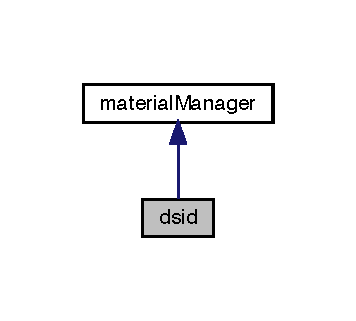
\includegraphics[width=171pt]{classdsid__inherit__graph}
\end{center}
\end{figure}


Collaboration diagram for dsid\+:
\nopagebreak
\begin{figure}[H]
\begin{center}
\leavevmode
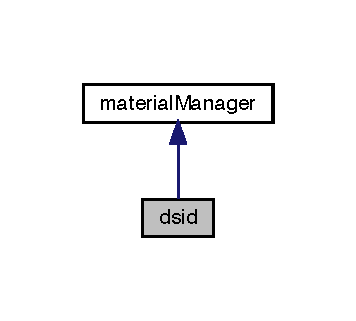
\includegraphics[width=171pt]{classdsid__coll__graph}
\end{center}
\end{figure}
\subsection*{Public Member Functions}
\begin{DoxyCompactItemize}
\item 
\mbox{\Hypertarget{classdsid_af56f1cb60f8a6d3c05ca03f08903fd9c}\label{classdsid_af56f1cb60f8a6d3c05ca03f08903fd9c}} 
{\bfseries dsid} (double E0, double Poisson0, double a1, double a2, double a3, double a4, double C0, double C1, double alpha, double Debug)
\item 
\mbox{\Hypertarget{classdsid_a2a80c33f9ab37eaa2668ba2babf2085d}\label{classdsid_a2a80c33f9ab37eaa2668ba2babf2085d}} 
void {\bfseries update} (r1\+Tensor$<$ double $>$ \&stn\+E\+\_\+, r1\+Tensor$<$ double $>$ \&stn\+S\+\_\+, r1\+Tensor$<$ double $>$ \&stn\+O\+\_\+, double \&fd0)
\item 
\mbox{\Hypertarget{classdsid_a7710e2004a4704ed03eaa9b196bf183d}\label{classdsid_a7710e2004a4704ed03eaa9b196bf183d}} 
void {\bfseries print\+Variables} ()
\end{DoxyCompactItemize}


The documentation for this class was generated from the following files\+:\begin{DoxyCompactItemize}
\item 
/\+Users/haoxu/\+Documents/git/\+Omega/src/constitutive/damage/\hyperlink{dsid_8h}{dsid.\+h}\item 
/\+Users/haoxu/\+Documents/git/\+Omega/src/constitutive/damage/dsid.\+cpp\end{DoxyCompactItemize}

\hypertarget{structedge}{}\section{edge Struct Reference}
\label{structedge}\index{edge@{edge}}
\subsection*{Public Member Functions}
\begin{DoxyCompactItemize}
\item 
\mbox{\Hypertarget{structedge_a4c39c242fee0455dc59703f16e5282a9}\label{structedge_a4c39c242fee0455dc59703f16e5282a9}} 
{\bfseries edge} (int n, r1\+Tensor$<$ \hyperlink{structnode}{node} $\ast$$>$ \&node\+Lists)
\item 
\mbox{\Hypertarget{structedge_a624447f195829a42deab34bfd980e99b}\label{structedge_a624447f195829a42deab34bfd980e99b}} 
{\bfseries edge} (const \hyperlink{structedge}{edge} \&rhs)
\item 
\mbox{\Hypertarget{structedge_aca7688959137a0e5449b415c0bc156f0}\label{structedge_aca7688959137a0e5449b415c0bc156f0}} 
void {\bfseries copy} (const \hyperlink{structedge}{edge} \&rhs)
\item 
\mbox{\Hypertarget{structedge_a009ea06571de93edd23e27add2bdc277}\label{structedge_a009ea06571de93edd23e27add2bdc277}} 
void {\bfseries distance} ()
\item 
\mbox{\Hypertarget{structedge_ae75be787e5efdbdfbb29b73a6676ce99}\label{structedge_ae75be787e5efdbdfbb29b73a6676ce99}} 
void {\bfseries reassign} (int n, r1\+Tensor$<$ \hyperlink{structnode}{node} $>$ \&node\+Lists)
\end{DoxyCompactItemize}
\subsection*{Public Attributes}
\begin{DoxyCompactItemize}
\item 
\mbox{\Hypertarget{structedge_a4d9067f195e1b95f485d6658d4797fda}\label{structedge_a4d9067f195e1b95f485d6658d4797fda}} 
int {\bfseries index}
\item 
\mbox{\Hypertarget{structedge_a19e3d41eb6833e846f44a01269cc0a8a}\label{structedge_a19e3d41eb6833e846f44a01269cc0a8a}} 
int {\bfseries n\+\_\+nodes}
\item 
\mbox{\Hypertarget{structedge_a64c18e8101ab904712ee054f9815dbf4}\label{structedge_a64c18e8101ab904712ee054f9815dbf4}} 
r1\+Tensor$<$ \hyperlink{structnode}{node} $\ast$ $>$ {\bfseries nodes}
\item 
\mbox{\Hypertarget{structedge_aceb28a0abbb66cdd04581b9be2660cca}\label{structedge_aceb28a0abbb66cdd04581b9be2660cca}} 
double {\bfseries dist}
\end{DoxyCompactItemize}


The documentation for this struct was generated from the following file\+:\begin{DoxyCompactItemize}
\item 
/\+Users/haoxu/\+Documents/git/element/edge.\+h\end{DoxyCompactItemize}

\hypertarget{classelement_manager}{}\section{element\+Manager Class Reference}
\label{classelement_manager}\index{element\+Manager@{element\+Manager}}
\subsection*{Public Member Functions}
\begin{DoxyCompactItemize}
\item 
\mbox{\Hypertarget{classelement_manager_ab15c1e207de0878fc5bc547f27805df6}\label{classelement_manager_ab15c1e207de0878fc5bc547f27805df6}} 
{\bfseries element\+Manager} (int m)
\item 
\mbox{\Hypertarget{classelement_manager_adb46d4ca8457958af02497fd231fd606}\label{classelement_manager_adb46d4ca8457958af02497fd231fd606}} 
{\bfseries element\+Manager} (std\+::string n)
\item 
\mbox{\Hypertarget{classelement_manager_a9f3bb87b33a55f480bdf65804fc77af7}\label{classelement_manager_a9f3bb87b33a55f480bdf65804fc77af7}} 
void {\bfseries assign} ()
\item 
\mbox{\Hypertarget{classelement_manager_a16cf4204e230aa2f3cc8cc7c79ab1363}\label{classelement_manager_a16cf4204e230aa2f3cc8cc7c79ab1363}} 
void {\bfseries update} ()
\end{DoxyCompactItemize}


The documentation for this class was generated from the following files\+:\begin{DoxyCompactItemize}
\item 
/\+Users/haoxu/\+Documents/git/\+Omega/src/class\+Manager/\hyperlink{element_manager_8h}{element\+Manager.\+h}\item 
/\+Users/haoxu/\+Documents/git/\+Omega/src/class\+Manager/element\+Manager.\+cpp\end{DoxyCompactItemize}

\hypertarget{classisotropic_elastic}{}\section{isotropic\+Elastic Class Reference}
\label{classisotropic_elastic}\index{isotropic\+Elastic@{isotropic\+Elastic}}


Inheritance diagram for isotropic\+Elastic\+:\nopagebreak
\begin{figure}[H]
\begin{center}
\leavevmode
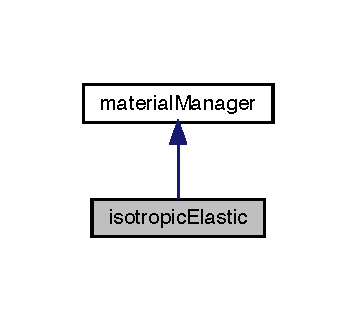
\includegraphics[width=171pt]{classisotropic_elastic__inherit__graph}
\end{center}
\end{figure}


Collaboration diagram for isotropic\+Elastic\+:\nopagebreak
\begin{figure}[H]
\begin{center}
\leavevmode
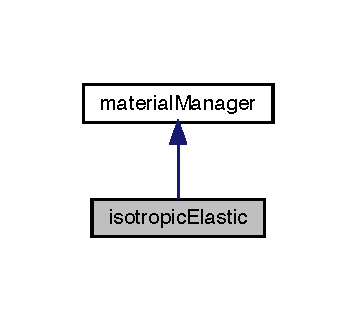
\includegraphics[width=171pt]{classisotropic_elastic__coll__graph}
\end{center}
\end{figure}
\subsection*{Public Member Functions}
\begin{DoxyCompactItemize}
\item 
\mbox{\Hypertarget{classisotropic_elastic_ab3b2f2897d0174e6b7feb44bbc498699}\label{classisotropic_elastic_ab3b2f2897d0174e6b7feb44bbc498699}} 
{\bfseries isotropic\+Elastic} (double youngs\+Modulus, double poissons\+Ratio)
\item 
\mbox{\Hypertarget{classisotropic_elastic_aa92c83e227328632cc01bf9223b95805}\label{classisotropic_elastic_aa92c83e227328632cc01bf9223b95805}} 
void {\bfseries update} (r1\+Tensor$<$ double $>$ \&strain\+Inc, r1\+Tensor$<$ double $>$ \&stress\+Inc)
\item 
\mbox{\Hypertarget{classisotropic_elastic_aced4646179b73c77af191c6716ea32d0}\label{classisotropic_elastic_aced4646179b73c77af191c6716ea32d0}} 
void {\bfseries print\+Variables} ()
\end{DoxyCompactItemize}


The documentation for this class was generated from the following files\+:\begin{DoxyCompactItemize}
\item 
/\+Users/haoxu/\+Documents/git/\+Omega/src/constitutive/elastic/\hyperlink{isotropic_elastic_8h}{isotropic\+Elastic.\+h}\item 
/\+Users/haoxu/\+Documents/git/\+Omega/src/constitutive/elastic/isotropic\+Elastic.\+cpp\end{DoxyCompactItemize}

\hypertarget{classmaterial_manager}{}\section{material\+Manager Class Reference}
\label{classmaterial_manager}\index{material\+Manager@{material\+Manager}}


Inheritance diagram for material\+Manager\+:
\nopagebreak
\begin{figure}[H]
\begin{center}
\leavevmode
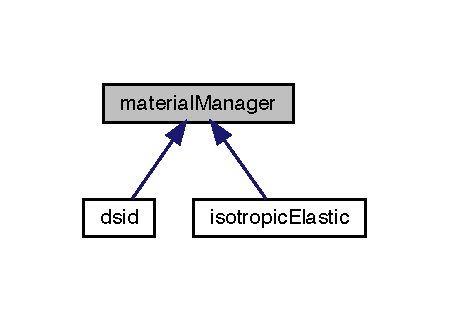
\includegraphics[width=216pt]{classmaterial_manager__inherit__graph}
\end{center}
\end{figure}
\subsection*{Public Member Functions}
\begin{DoxyCompactItemize}
\item 
\mbox{\Hypertarget{classmaterial_manager_a7115733155d4980fb064ad2aba49f3b6}\label{classmaterial_manager_a7115733155d4980fb064ad2aba49f3b6}} 
{\bfseries material\+Manager} (int m)
\item 
\mbox{\Hypertarget{classmaterial_manager_ac16268d521521df8030d7ab083f154b0}\label{classmaterial_manager_ac16268d521521df8030d7ab083f154b0}} 
{\bfseries material\+Manager} (std\+::string n)
\item 
\mbox{\Hypertarget{classmaterial_manager_a7caaa224d43ed192b5a7cbcbad75d2ae}\label{classmaterial_manager_a7caaa224d43ed192b5a7cbcbad75d2ae}} 
void {\bfseries assign} ()
\item 
\mbox{\Hypertarget{classmaterial_manager_a457cc335abb8e90f97a6a046b95d1162}\label{classmaterial_manager_a457cc335abb8e90f97a6a046b95d1162}} 
virtual void {\bfseries update} ()
\end{DoxyCompactItemize}


The documentation for this class was generated from the following files\+:\begin{DoxyCompactItemize}
\item 
/\+Users/haoxu/\+Documents/git/\+Omega/src/class\+Manager/\hyperlink{material_manager_8h}{material\+Manager.\+h}\item 
/\+Users/haoxu/\+Documents/git/\+Omega/src/class\+Manager/material\+Manager.\+cpp\end{DoxyCompactItemize}

\hypertarget{structnode}{}\section{node Struct Reference}
\label{structnode}\index{node@{node}}
\subsection*{Public Member Functions}
\begin{DoxyCompactItemize}
\item 
\mbox{\Hypertarget{structnode_ad19e263fcbe5d2ffec70b40818c6dc10}\label{structnode_ad19e263fcbe5d2ffec70b40818c6dc10}} 
{\bfseries node} (int n=0, double x=0., double y=0., double z=0.)
\item 
\mbox{\Hypertarget{structnode_a1598c2f405acda6b1505be2a727b2cce}\label{structnode_a1598c2f405acda6b1505be2a727b2cce}} 
{\bfseries node} (int n, r1\+Tensor$<$ double $>$ \&coord)
\item 
\mbox{\Hypertarget{structnode_a6849162e873f597d90609d00a141f98d}\label{structnode_a6849162e873f597d90609d00a141f98d}} 
{\bfseries node} (const \hyperlink{structnode}{node} \&rhs)
\item 
\mbox{\Hypertarget{structnode_a8ae2ec6f78a4989965068e15d8253e9b}\label{structnode_a8ae2ec6f78a4989965068e15d8253e9b}} 
void {\bfseries copy} (const \hyperlink{structnode}{node} \&rhs)
\end{DoxyCompactItemize}
\subsection*{Public Attributes}
\begin{DoxyCompactItemize}
\item 
\mbox{\Hypertarget{structnode_a5359a7ce1309be9415907be3ebbd2f91}\label{structnode_a5359a7ce1309be9415907be3ebbd2f91}} 
int {\bfseries index}
\item 
\mbox{\Hypertarget{structnode_ad17f1c5ff47a87b556076964100ae29f}\label{structnode_ad17f1c5ff47a87b556076964100ae29f}} 
double {\bfseries xx}
\item 
\mbox{\Hypertarget{structnode_ae028aef81870b46c0bc9b348ba8fcd64}\label{structnode_ae028aef81870b46c0bc9b348ba8fcd64}} 
double {\bfseries yy}
\item 
\mbox{\Hypertarget{structnode_a0190e7bd9d3cffe85e91d2310bd49ca0}\label{structnode_a0190e7bd9d3cffe85e91d2310bd49ca0}} 
double {\bfseries zz}
\end{DoxyCompactItemize}


The documentation for this struct was generated from the following file\+:\begin{DoxyCompactItemize}
\item 
/\+Users/haoxu/\+Documents/git/element/node.\+h\end{DoxyCompactItemize}

\hypertarget{classsolver_manager}{}\section{solver\+Manager Class Reference}
\label{classsolver_manager}\index{solver\+Manager@{solver\+Manager}}
\subsection*{Public Member Functions}
\begin{DoxyCompactItemize}
\item 
\mbox{\Hypertarget{classsolver_manager_a4b54a1ebc362bb24bf3bad19ecd4dfc9}\label{classsolver_manager_a4b54a1ebc362bb24bf3bad19ecd4dfc9}} 
{\bfseries solver\+Manager} (int m)
\item 
\mbox{\Hypertarget{classsolver_manager_af8f807bfa004a9cdc9adf3febd467173}\label{classsolver_manager_af8f807bfa004a9cdc9adf3febd467173}} 
{\bfseries solver\+Manager} (std\+::string n)
\item 
\mbox{\Hypertarget{classsolver_manager_af748e8337f584a287021659236ce0946}\label{classsolver_manager_af748e8337f584a287021659236ce0946}} 
void {\bfseries assign} ()
\item 
\mbox{\Hypertarget{classsolver_manager_a96e9e5db3a690dcfec3428f4deca2a5b}\label{classsolver_manager_a96e9e5db3a690dcfec3428f4deca2a5b}} 
void {\bfseries update} ()
\end{DoxyCompactItemize}


The documentation for this class was generated from the following files\+:\begin{DoxyCompactItemize}
\item 
/\+Users/haoxu/\+Documents/git/\+Omega/src/class\+Manager/\hyperlink{solver_manager_8h}{solver\+Manager.\+h}\item 
/\+Users/haoxu/\+Documents/git/\+Omega/src/class\+Manager/solver\+Manager.\+cpp\end{DoxyCompactItemize}

\hypertarget{structsurface}{}\section{surface Struct Reference}
\label{structsurface}\index{surface@{surface}}
\subsection*{Public Member Functions}
\begin{DoxyCompactItemize}
\item 
\mbox{\Hypertarget{structsurface_afc5369f573afffc96aa9c47702467e9a}\label{structsurface_afc5369f573afffc96aa9c47702467e9a}} 
{\bfseries surface} (int n, r1\+Tensor$<$ \hyperlink{structnode}{node} $>$ \&node\+Lists)
\item 
\mbox{\Hypertarget{structsurface_ace2837a6697083d412f54f75831f5d4e}\label{structsurface_ace2837a6697083d412f54f75831f5d4e}} 
void {\bfseries area\+\_\+surf1} ()
\end{DoxyCompactItemize}
\subsection*{Public Attributes}
\begin{DoxyCompactItemize}
\item 
\mbox{\Hypertarget{structsurface_a2982d55d5c6a8b5e2473987c0613d302}\label{structsurface_a2982d55d5c6a8b5e2473987c0613d302}} 
int {\bfseries index}
\item 
\mbox{\Hypertarget{structsurface_a6e23728322497ca185edbb2ebee2bc0d}\label{structsurface_a6e23728322497ca185edbb2ebee2bc0d}} 
int {\bfseries n\+\_\+nodes}
\item 
\mbox{\Hypertarget{structsurface_af41fd81f0ab34fee9617c23737876f4e}\label{structsurface_af41fd81f0ab34fee9617c23737876f4e}} 
int {\bfseries n\+\_\+edges}
\item 
\mbox{\Hypertarget{structsurface_a16ab1fdfe574000a606add5ab5f1a924}\label{structsurface_a16ab1fdfe574000a606add5ab5f1a924}} 
r1\+Tensor$<$ \hyperlink{structnode}{node} $\ast$ $>$ {\bfseries nodes}
\item 
\mbox{\Hypertarget{structsurface_aeb700efb2047a0c346e5016d15ef5151}\label{structsurface_aeb700efb2047a0c346e5016d15ef5151}} 
r1\+Tensor$<$ \hyperlink{structedge}{edge} $>$ {\bfseries edges}
\item 
\mbox{\Hypertarget{structsurface_a2ea0783fd4be9a6ed18cff9008c6e3f0}\label{structsurface_a2ea0783fd4be9a6ed18cff9008c6e3f0}} 
double {\bfseries area}
\item 
\mbox{\Hypertarget{structsurface_a16d25b4e0851e4a36c974b1fdb2f63a0}\label{structsurface_a16d25b4e0851e4a36c974b1fdb2f63a0}} 
int {\bfseries kind}
\end{DoxyCompactItemize}


The documentation for this struct was generated from the following file\+:\begin{DoxyCompactItemize}
\item 
/\+Users/haoxu/\+Documents/git/element/surface.\+h\end{DoxyCompactItemize}

\hypertarget{classtask_manager}{}\section{task\+Manager Class Reference}
\label{classtask_manager}\index{task\+Manager@{task\+Manager}}
\subsection*{Public Member Functions}
\begin{DoxyCompactItemize}
\item 
\mbox{\Hypertarget{classtask_manager_a034bd43127331a49e48593147aa7cda3}\label{classtask_manager_a034bd43127331a49e48593147aa7cda3}} 
{\bfseries task\+Manager} (int m)
\item 
\mbox{\Hypertarget{classtask_manager_abd6f35d4dd5ad8f18f60886ba7b52e25}\label{classtask_manager_abd6f35d4dd5ad8f18f60886ba7b52e25}} 
void {\bfseries print} ()
\item 
\mbox{\Hypertarget{classtask_manager_a119e482c8acafa770568ba8578445ca5}\label{classtask_manager_a119e482c8acafa770568ba8578445ca5}} 
void {\bfseries initialize} (int \&argc, char $\ast$$\ast$\&argv)
\item 
\mbox{\Hypertarget{classtask_manager_a8d8797b3bc3691ccf7f6445e05c0f34e}\label{classtask_manager_a8d8797b3bc3691ccf7f6445e05c0f34e}} 
void {\bfseries get\+Options} (int \&argc, char $\ast$$\ast$\&argv)
\item 
\mbox{\Hypertarget{classtask_manager_a584d4e55b58302308fd2d15f7ffd43c9}\label{classtask_manager_a584d4e55b58302308fd2d15f7ffd43c9}} 
void {\bfseries assemble} ()
\item 
\mbox{\Hypertarget{classtask_manager_abef65e91b2ac2969750d0cf6979be684}\label{classtask_manager_abef65e91b2ac2969750d0cf6979be684}} 
void {\bfseries run} ()
\item 
\mbox{\Hypertarget{classtask_manager_a7cc568b0a99bc06adaa1938f38e0fb7f}\label{classtask_manager_a7cc568b0a99bc06adaa1938f38e0fb7f}} 
void {\bfseries post\+Process} ()
\end{DoxyCompactItemize}


The documentation for this class was generated from the following files\+:\begin{DoxyCompactItemize}
\item 
/\+Users/haoxu/\+Documents/git/\+Omega/src/class\+Manager/\hyperlink{task_manager_8h}{task\+Manager.\+h}\item 
/\+Users/haoxu/\+Documents/git/\+Omega/src/class\+Manager/task\+Manager.\+cpp\end{DoxyCompactItemize}

\chapter{File Documentation}
\hypertarget{element_manager_8h}{}\section{/\+Users/haoxu/\+Documents/git/\+Omega/src/class\+Manager/element\+Manager.h File Reference}
\label{element_manager_8h}\index{/\+Users/haoxu/\+Documents/git/\+Omega/src/class\+Manager/element\+Manager.\+h@{/\+Users/haoxu/\+Documents/git/\+Omega/src/class\+Manager/element\+Manager.\+h}}
{\ttfamily \#include $<$iostream$>$}\newline
{\ttfamily \#include $<$string$>$}\newline
Include dependency graph for element\+Manager.\+h\+:
\nopagebreak
\begin{figure}[H]
\begin{center}
\leavevmode
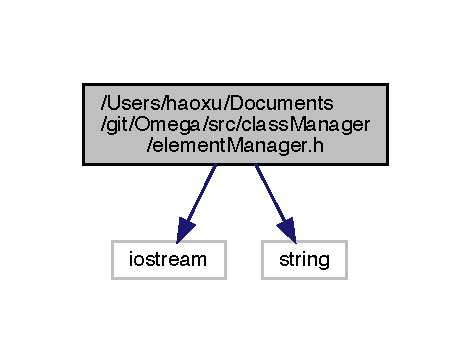
\includegraphics[width=226pt]{element_manager_8h__incl}
\end{center}
\end{figure}
This graph shows which files directly or indirectly include this file\+:
\nopagebreak
\begin{figure}[H]
\begin{center}
\leavevmode
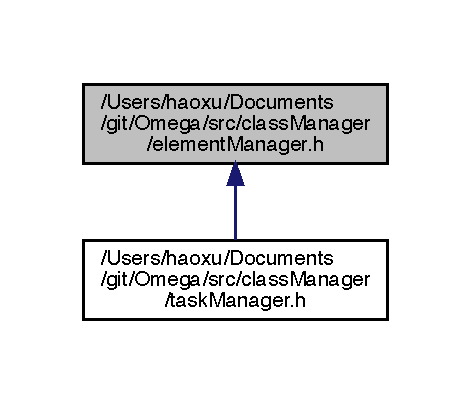
\includegraphics[width=226pt]{element_manager_8h__dep__incl}
\end{center}
\end{figure}
\subsection*{Classes}
\begin{DoxyCompactItemize}
\item 
class \hyperlink{classelement_manager}{element\+Manager}
\end{DoxyCompactItemize}


\subsection{Detailed Description}
\begin{DoxyAuthor}{Author}
Hao Xu 
\end{DoxyAuthor}
\begin{DoxyDate}{Date}
created on 2017/07/21 
\end{DoxyDate}

\hypertarget{material_manager_8h}{}\section{/\+Users/haoxu/\+Documents/git/\+Omega/src/class\+Manager/material\+Manager.h File Reference}
\label{material_manager_8h}\index{/\+Users/haoxu/\+Documents/git/\+Omega/src/class\+Manager/material\+Manager.\+h@{/\+Users/haoxu/\+Documents/git/\+Omega/src/class\+Manager/material\+Manager.\+h}}
{\ttfamily \#include $<$iostream$>$}\newline
{\ttfamily \#include $<$string$>$}\newline
Include dependency graph for material\+Manager.\+h\+:
\nopagebreak
\begin{figure}[H]
\begin{center}
\leavevmode
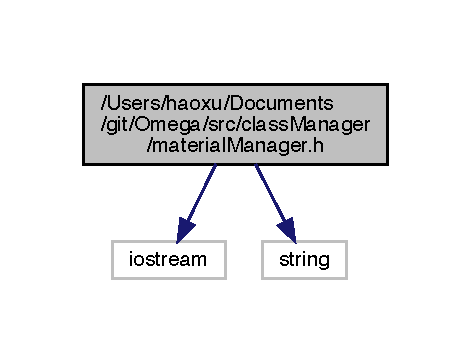
\includegraphics[width=226pt]{material_manager_8h__incl}
\end{center}
\end{figure}
This graph shows which files directly or indirectly include this file\+:
\nopagebreak
\begin{figure}[H]
\begin{center}
\leavevmode
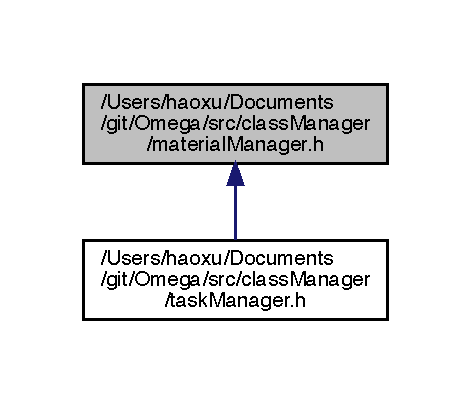
\includegraphics[width=226pt]{material_manager_8h__dep__incl}
\end{center}
\end{figure}
\subsection*{Classes}
\begin{DoxyCompactItemize}
\item 
class \hyperlink{classmaterial_manager}{material\+Manager}
\end{DoxyCompactItemize}


\subsection{Detailed Description}
\begin{DoxyAuthor}{Author}
Hao Xu 
\end{DoxyAuthor}
\begin{DoxyDate}{Date}
created on 2017/07/21 
\end{DoxyDate}

\hypertarget{solver_manager_8h}{}\section{/\+Users/haoxu/\+Documents/git/\+Omega/src/class\+Manager/solver\+Manager.h File Reference}
\label{solver_manager_8h}\index{/\+Users/haoxu/\+Documents/git/\+Omega/src/class\+Manager/solver\+Manager.\+h@{/\+Users/haoxu/\+Documents/git/\+Omega/src/class\+Manager/solver\+Manager.\+h}}
{\ttfamily \#include $<$iostream$>$}\newline
{\ttfamily \#include $<$string$>$}\newline
Include dependency graph for solver\+Manager.\+h\+:\nopagebreak
\begin{figure}[H]
\begin{center}
\leavevmode
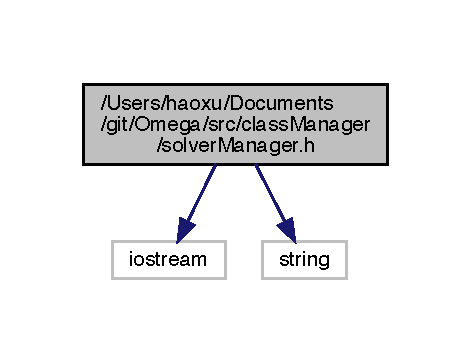
\includegraphics[width=226pt]{solver_manager_8h__incl}
\end{center}
\end{figure}
This graph shows which files directly or indirectly include this file\+:\nopagebreak
\begin{figure}[H]
\begin{center}
\leavevmode
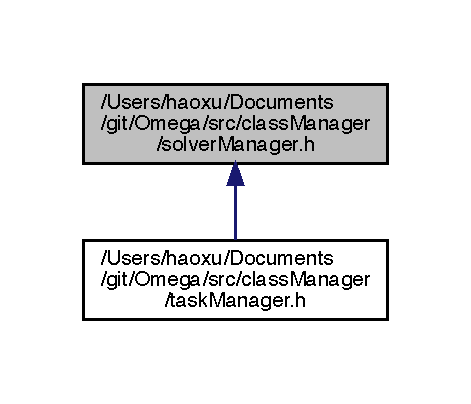
\includegraphics[width=226pt]{solver_manager_8h__dep__incl}
\end{center}
\end{figure}
\subsection*{Classes}
\begin{DoxyCompactItemize}
\item 
class \hyperlink{classsolver_manager}{solver\+Manager}
\end{DoxyCompactItemize}


\subsection{Detailed Description}
\begin{DoxyAuthor}{Author}
Hao Xu 
\end{DoxyAuthor}
\begin{DoxyDate}{Date}
created on 2017/07/21 
\end{DoxyDate}

\hypertarget{task_manager_8h}{}\section{/\+Users/haoxu/\+Documents/git/\+Omega/src/class\+Manager/task\+Manager.h File Reference}
\label{task_manager_8h}\index{/\+Users/haoxu/\+Documents/git/\+Omega/src/class\+Manager/task\+Manager.\+h@{/\+Users/haoxu/\+Documents/git/\+Omega/src/class\+Manager/task\+Manager.\+h}}
{\ttfamily \#include $<$iostream$>$}\newline
{\ttfamily \#include $<$vector$>$}\newline
{\ttfamily \#include $<$getopt.\+h$>$}\newline
{\ttfamily \#include \char`\"{}mpi.\+h\char`\"{}}\newline
{\ttfamily \#include \char`\"{}tinyxml2/tinyxml2.\+h\char`\"{}}\newline
{\ttfamily \#include \char`\"{}element\+Manager.\+h\char`\"{}}\newline
{\ttfamily \#include \char`\"{}material\+Manager.\+h\char`\"{}}\newline
{\ttfamily \#include \char`\"{}solver\+Manager.\+h\char`\"{}}\newline
Include dependency graph for task\+Manager.\+h\+:\nopagebreak
\begin{figure}[H]
\begin{center}
\leavevmode
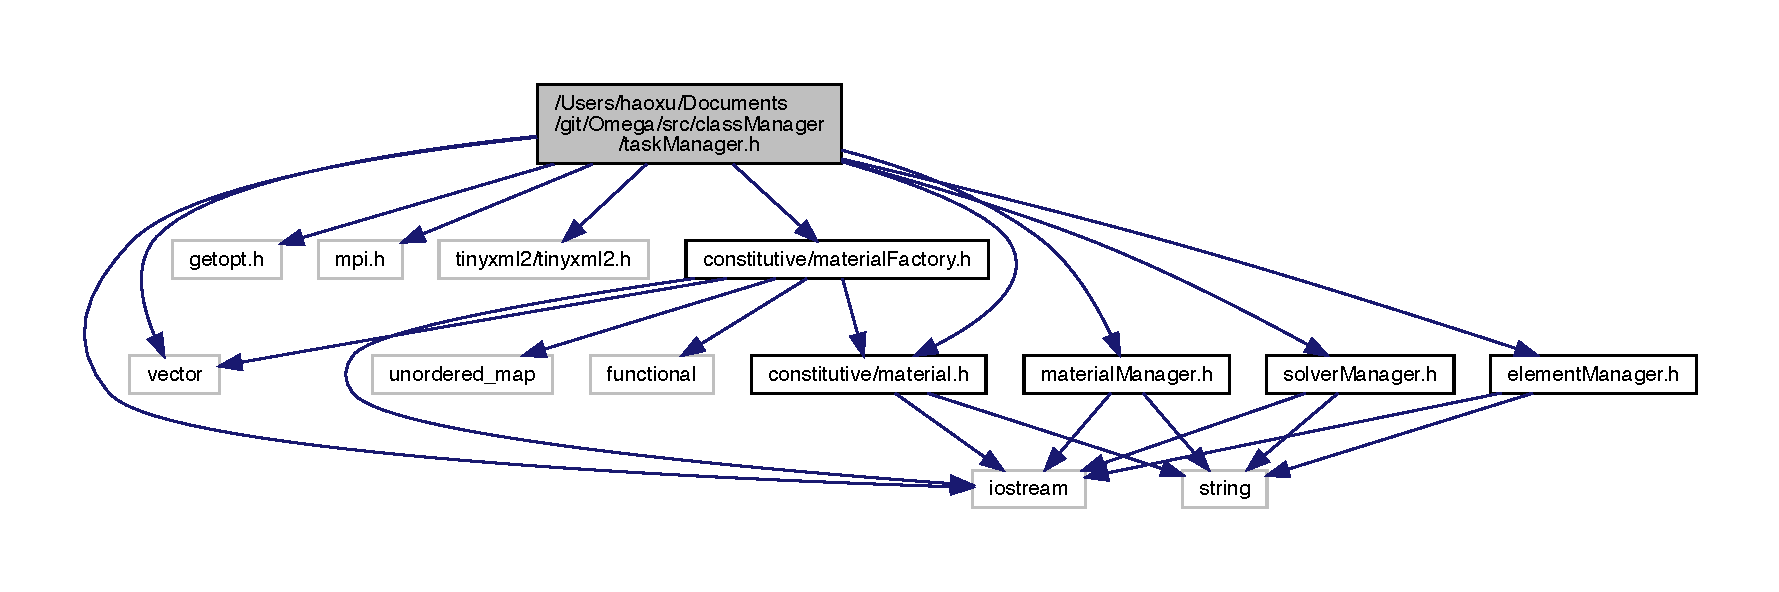
\includegraphics[width=350pt]{task_manager_8h__incl}
\end{center}
\end{figure}
\subsection*{Classes}
\begin{DoxyCompactItemize}
\item 
class \hyperlink{classtask_manager}{task\+Manager}
\end{DoxyCompactItemize}


\subsection{Detailed Description}
\begin{DoxyAuthor}{Author}
Hao Xu 
\end{DoxyAuthor}
\begin{DoxyDate}{Date}
created on 2017/07/21 
\end{DoxyDate}

\hypertarget{dsid_8h}{}\section{/\+Users/haoxu/\+Documents/git/\+Omega/src/constitutive/damage/dsid.h File Reference}
\label{dsid_8h}\index{/\+Users/haoxu/\+Documents/git/\+Omega/src/constitutive/damage/dsid.\+h@{/\+Users/haoxu/\+Documents/git/\+Omega/src/constitutive/damage/dsid.\+h}}
{\ttfamily \#include \char`\"{}lib/math\+Lib/r1\+Tensor.\+h\char`\"{}}\newline
{\ttfamily \#include \char`\"{}lib/math\+Lib/r2\+Tensor.\+h\char`\"{}}\newline
{\ttfamily \#include \char`\"{}lib/math\+Lib/r3\+Tensor.\+h\char`\"{}}\newline
Include dependency graph for dsid.\+h\+:\nopagebreak
\begin{figure}[H]
\begin{center}
\leavevmode
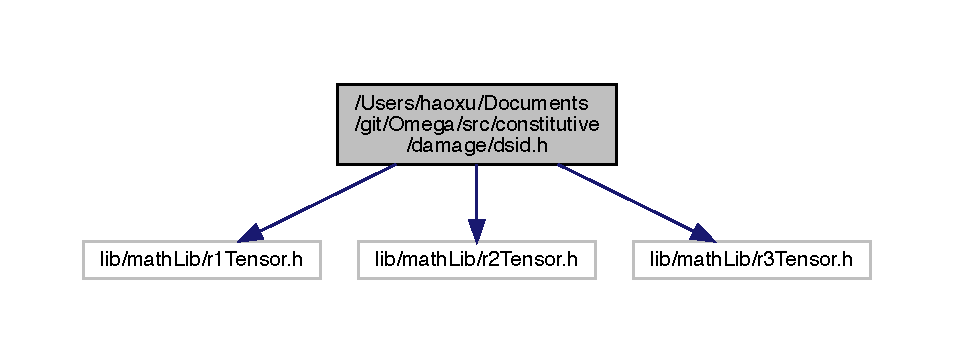
\includegraphics[width=350pt]{dsid_8h__incl}
\end{center}
\end{figure}
\subsection*{Classes}
\begin{DoxyCompactItemize}
\item 
class \hyperlink{classdsid}{dsid}
\end{DoxyCompactItemize}


\subsection{Detailed Description}
\begin{DoxyAuthor}{Author}
Hao Xu 
\end{DoxyAuthor}
\begin{DoxyDate}{Date}
created on 2017/07/21 
\end{DoxyDate}

\hypertarget{isotropic_elastic_8h}{}\section{/\+Users/haoxu/\+Documents/git/\+Omega/src/constitutive/elastic/isotropic\+Elastic.h File Reference}
\label{isotropic_elastic_8h}\index{/\+Users/haoxu/\+Documents/git/\+Omega/src/constitutive/elastic/isotropic\+Elastic.\+h@{/\+Users/haoxu/\+Documents/git/\+Omega/src/constitutive/elastic/isotropic\+Elastic.\+h}}
{\ttfamily \#include \char`\"{}lib/math\+Lib/r1\+Tensor.\+h\char`\"{}}\newline
{\ttfamily \#include \char`\"{}lib/math\+Lib/r2\+Tensor.\+h\char`\"{}}\newline
{\ttfamily \#include \char`\"{}lib/math\+Lib/r3\+Tensor.\+h\char`\"{}}\newline
Include dependency graph for isotropic\+Elastic.\+h\+:\nopagebreak
\begin{figure}[H]
\begin{center}
\leavevmode
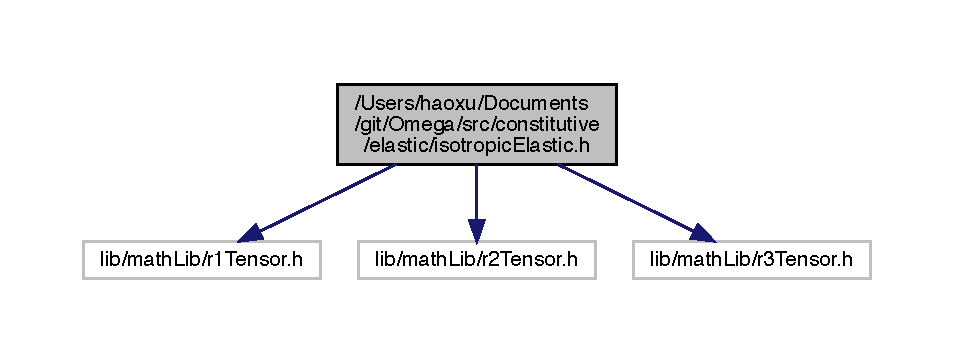
\includegraphics[width=350pt]{isotropic_elastic_8h__incl}
\end{center}
\end{figure}
\subsection*{Classes}
\begin{DoxyCompactItemize}
\item 
class \hyperlink{classisotropic_elastic}{isotropic\+Elastic}
\end{DoxyCompactItemize}


\subsection{Detailed Description}
\begin{DoxyAuthor}{Author}
Hao Xu 
\end{DoxyAuthor}
\begin{DoxyDate}{Date}
created on 2017/07/21 
\end{DoxyDate}

%--- End generated contents ---

% Index
\backmatter
\newpage
\phantomsection
\clearemptydoublepage
\addcontentsline{toc}{chapter}{Index}
\printindex

\end{document}
